\def\timpInainteDeRay{0}
\def\timpDupaRay{0}

\chapter{Arhitectura aplicației}
\section{Împărțirea codului}
Codul este împărțit în 4 clase diferite. Ele au rolul de a forma un pipeline ce primește ca input fișiere în format csv, împreună cu montura electrozilor și ca rezultat oferă obiecte în formatul librăriei MNE.
În total, pipeline-ul meu este format din 5 clase: EEGPipelineOptions, EEGSubjectPipeline, EEGDataLoader, EEGPreprocessor și EEGEpochedData. 

Prima dată, opțiunile de preprocesare și de formatare în epoci sunt setate utilizând EEGPipelineOptions. Acest obiect este trimis mai departe către EEGSubjectPipeline. Aici, este orchestrat restul pipeline-ului în felul următor: datele din format .csv sunt transformate în format .fif(compatibil cu MNE) utilizând EEGDataLoader. Datele în format .fif sunt transformate în date de forma mne.Raw(semnalul întreg, nesegmentat). Aici sunt totodată și preprocesate utilizând filtrul bandpass, ICA, interpolarea, și/sau, opțional, normalizare și scalare în intervalul [0, 1].  Ultimul pas îl reprezintă EEGEpochedData, unde semnalul Raw este segmentat în epoci. În funcție de opțiunile alese, aici poate fi aplciat și algoritmul de AutoReject pentru a scăpa de epocile corupte. Totodată, în această clasă este situată și funcția de extragere a setului de date, împreună cu labelul acestuia.


\section{Optimizarea încărcării datelor folosind Ray}
Pentru a încărca eficient cei 26 de participanți am utilizat librăria Ray\cite{Ray}. Ray este o librărie specializată în paralelizarea programelor Python, având ca scop principal programele din domeniul de Machine Learning. Modul de paralelizare a constat prin decorarea functiilor de încarcare a datelor cu @ray.remote și așteptarea rezultatului cu ray.get. Am folosit astfel toate cele 8 core-uri de care dispune calculatorul meu. De asemenea, timpul a fost redus de la $\timpInainteDeRay$ secunde la $\timpDupaRay$ secunde.

\setlength{\abovecaptionskip}{0pt}
\setlength{\belowcaptionskip}{0pt}
\clearpage
\begin{figure}[!h]
    \centering
    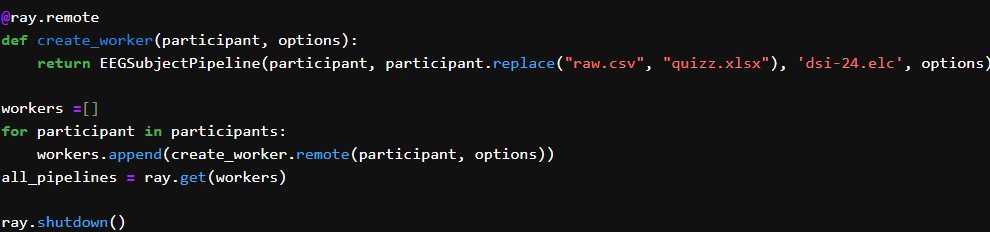
\includegraphics[width=1\linewidth]{images/ray.png}
    \caption{Paralelizare utilizând Ray}
    \label{fig:enter-label}
\end{figure}

\begin{figure}[h]
    \centering
    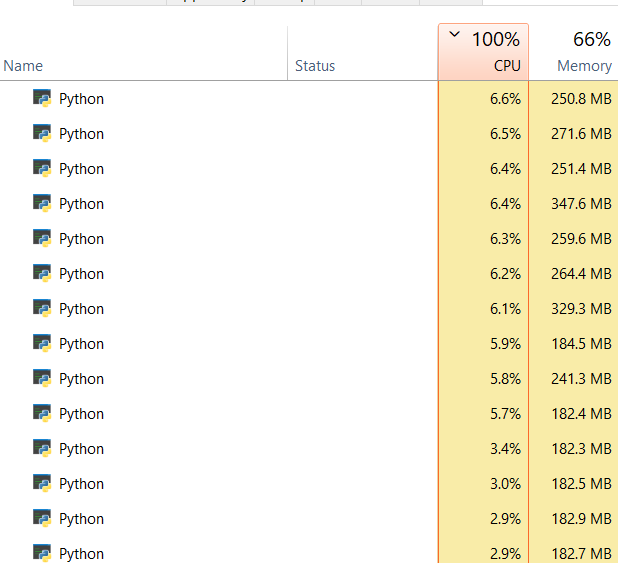
\includegraphics[width=0.7\linewidth]{task_manager.png}
    \caption{Load-ul pe calculator}
    \label{fig:enter-label}
\end{figure}